\section{Zadání}

Zvolte libovolný soubor dat z oblasti ekonometrického modelování.
Formulujte lineární model popisující vazby dat.
Odhadněte metodou nejmenších čtverců parametry modelu – odhad proveďte bodově i intervalově.
Zhodnoťte kvalitu modelu.
Proveďte základní regresní diagnostiku – identifikujte odlehlá a vlivná pozorování, proveďte testy residuí.

\section{Data}

Dataset byl vybrán z doporučené adresy \nolinkurl{http://pages.stern.nyu.edu/~wgreene/Text/Edition7/tablelist8new.htm}.
Konkrétně se jedná o set F4.1, data o prodeji Monetových obrazů.
Tento dataset obsahuje 430 pozorování a 6 příznaků.
Příznaky jsou cena [miliony USD] (vysvětlovaná proměnná), výška a šířka díla, binární příznak značící zda-li je dílo podepsáno (vysvětlující proměnné).
Dále jsou přítomny příznaky ID obrazu (pro identifikaci opakovaných prodejů) a kód aukčního domu, kde proběhla dražba.

\section{Vypracování}

Definicí lineárního modelu jsme se zabývali v minulé semestrální práci.
Pro vypracování této práce použijeme 3 vysvětlující proměnné (výšku, šířku obrazu a příznak podpisu) a vysvětlovanou proměnnou – prodejní cenu díla.
Výsledný regresní model nebude přímkový, nýbrž nadrovinný.

\begin{equation}
    Y_i = \beta_0 + \beta_1 X_i + \beta_2 X_i + \beta_3 X_i + \epsilon_i; \: i = 1,2,\ldots,n
\end{equation}

Bodový odhad parametrů modelu získáme pomocí funkce \textit{regress}.

\begin{equation}
    \hat{\beta} = \left[\begin{matrix} -4.6763 \\ 0.0902 \\ 0.1080 \\ 2.1989 \end{matrix}\right]
\end{equation}

Intervalový odhad parametrů taktéž.

\begin{equation}
    \hat{\beta}_{int} = \left[\begin{matrix} -6.3077 & -3.0449 \\ 0.0475 & 0.1330 \\ 0.0669 & 0.1490 \\ 1.2215 & 3.1764 \end{matrix}\right]
\end{equation}

Při konstrukci modelu lineární regrese nesmíme zapomenout na předpoklady, které dané konstrukci předcházejí:

\begin{enumerate}
    \item linearita,
    \item nezávislost reziduí,
    \item homoskedasticita,
    \item normalita reziduí.
\end{enumerate}

V případě, že máme více vysvětlujících proměnných, je z pohledu statistické inference též důležitá \textit{multikolinearita}.
To je předpoklad minimální, nebo žádné lineární závislosti mezi vysvětlujícími proměnnými.

Poslední důležitou položkou, která může pomoci při zhodnocení kvality modelu jsou pákové body.
Jejich počet a celkový vliv na model.

Graf~\ref{fig:lr1} ukazuje vztah vysvětlované proměnné na proměnných vysvětlujících.
Z grafu je možné vyčíst, že za větší částky se prodávají obrazy s autorovým podpisem.
Velikost obrazu nemá vliv na cenu ve smyslu přímé úměry.

\begin{figure}[htb]
    \centering
    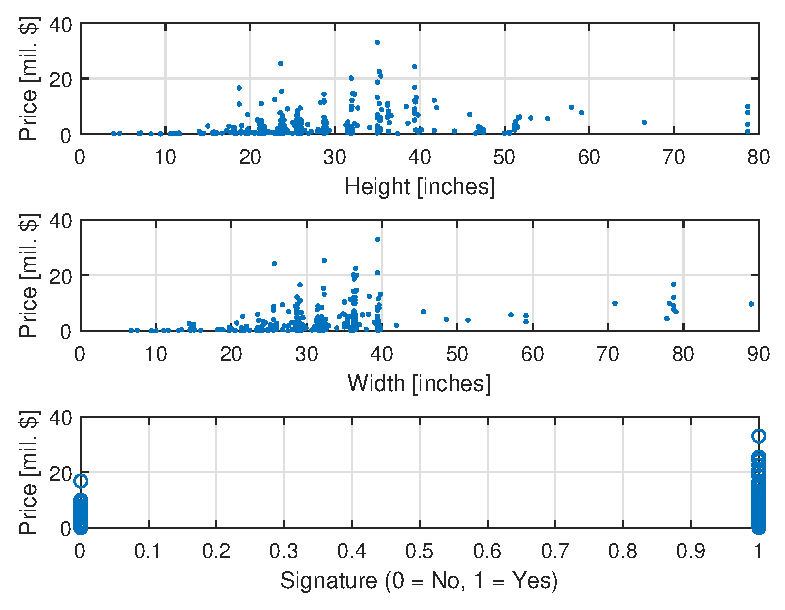
\includegraphics[width=0.55\textwidth]{graphs/fig1.eps}
    \caption{Vztah ceny a vysvětlujících proměnných}
    \label{fig:lr1}
\end{figure}
\FloatBarrier

Tou asi nejběžnější cestou, jak zkontrolovat lineární závislost v modelu (v případě více proměnných) je vykreslení preferovaně studentizovaných reziduí proti lineárně predikované proměnné.
Data jsou tímto způsobem vykreslena na grafu~\ref{fig:lr4}.
Vizuálním testem tvrdím, že lze data aproximovat polynomem prvního stupně, data jsou tedy správně predikována lineárním modelem.
Kdyby data byla rozložena ve tvaru nějaké výrazné křivky, naznačovalo by to volbu nesprávného modelu.

\begin{figure}[htb]
    \centering
    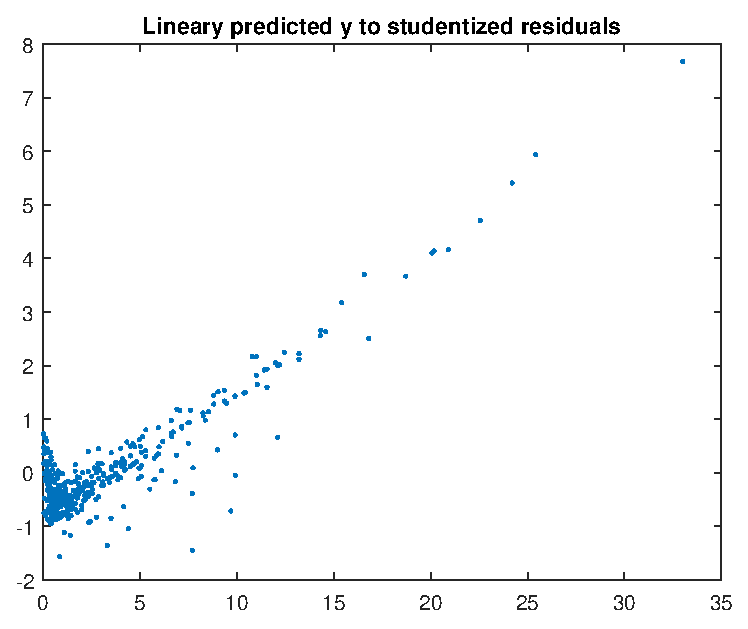
\includegraphics[width=0.55\textwidth]{graphs/fig4.eps}
    \caption{Zhodnocení linearity modelu}
    \label{fig:lr4}
\end{figure}
\FloatBarrier

Homoskedasticitu vyhodnotíme na základě číslených hodnot v přiloženém skriptu.
Pod proměnnou \textit{h} se skrývá výsledek 2-výběrového F-testu shody dvou rozptylů (v tomto případě dvou částí predikované proměnné).
Výsledek testu ukazuje, že rozptyly těchto částí jsou rozdílné, tedy data jsou zatížena heteroskedasticitou.

To přináší několik problémů.
Heteroskedasticita může zapříčinit nesprávný odhad parametrů modelu a může ovlivnit výsledky statistik.
Výsledky statistik ovlivňuje tak, že způsobuje nepřesnosti v evýpočtech p-hodnot.
P-hodnoty v datech zatížených tímto problémem bývají menší než ve skutečnosti a to v důsledku způsobuje, že zkoumaný jev může být označen za statisticky signofokantní, ačkoliv ve skutečnosti není.
Takže proč je v těchto datech heteroskedasticita?
Domnívám se, že se jedná o podstatu dat.
Výška, šířka obrazu a přítomnost autorova podpisu jsou sice zajímavými prediktory, absolutně však ignorují další faktory, jako např. historický podtext, které mohou mít vliv na finální prodejní cenu díla.
Tudíž se domnívám, že přítomná heteroskedasticita je tzv. \textit{pure} - čistá (\textit{impure} by byla způsobená chybným modelem) a není ji třeba v mém případě více řešit.

Na následujícím grafu lze zhodnotit normalitu reziduí.
Z grafu (a provedených testů normality ve skriptu) bohužel vyplývá, že rezidua nejsou normálně rozložená.
Dle článků, které jsem s ohledem na tento problém pročetl, není takový stav vážným problémem.
Problém bude pravděpodobně způsoben, obdobně jako u heteroskedasticity, nedostatečně reprezentativní formou vysvětlujících proměnných.
Domnívám se, že by pomohlo odstraněnní heteroskedasticity a pákových bodů.

\begin{figure}[htb]
    \centering
    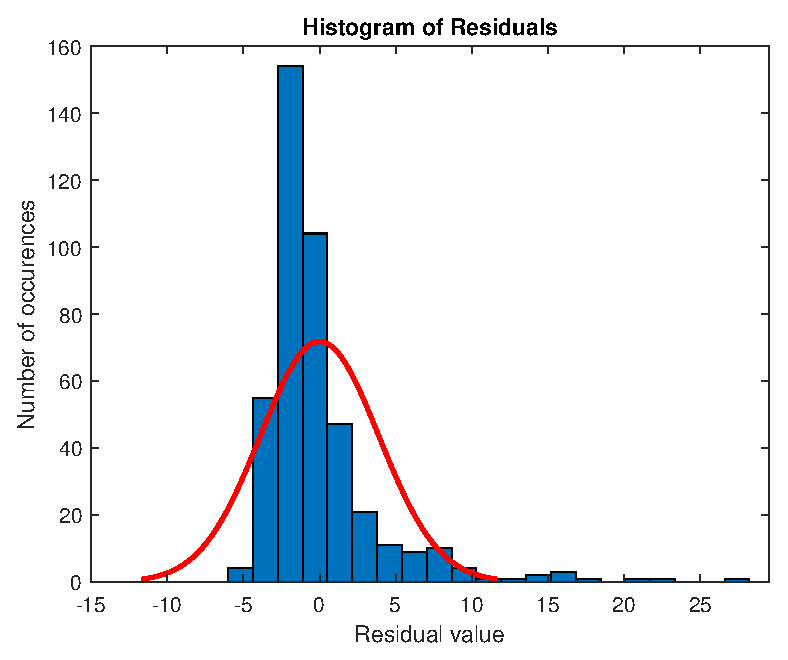
\includegraphics[width=0.55\textwidth]{graphs/fig3.eps}
    \caption{Normalita reziduí}
    \label{fig:lr3}
\end{figure}
\FloatBarrier

Pro detekci pákových bodů byly použity 3 metriky.
V závislosti na metrice bylo nalezeno 12-53 pákových bodů.
\( 12.3 \: \% \) pákových bodů je z pohledu analýzy asi celkem dost, ale zase je nutné přihlédnout k charakteru dat, jedná se o prodej uměleckých děl a lidský faktor vytváří v těchto případech hodně iregularit.
Pákové body vyhodnocené Cookovou vzdáleností jsou na grafu~\ref{fig:lr2}.

\begin{figure}[htb]
    \centering
    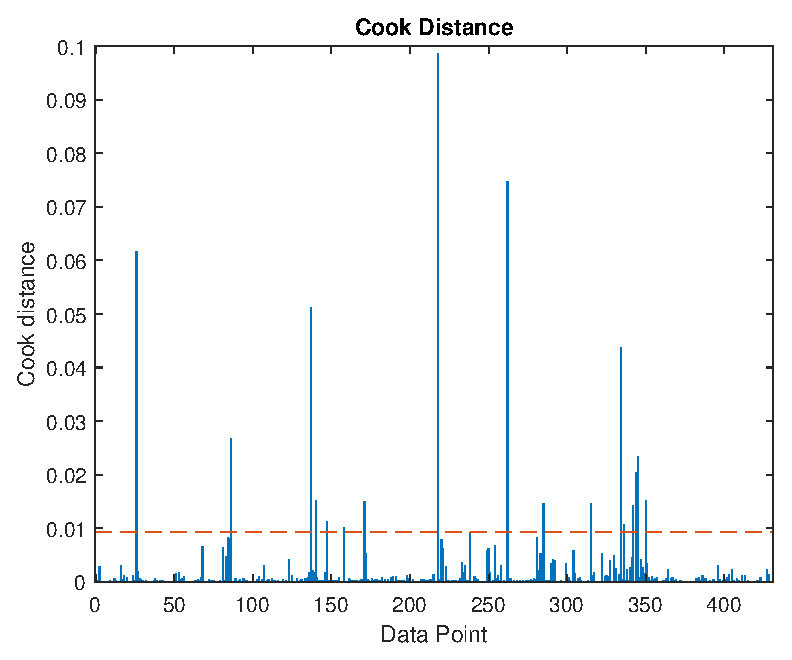
\includegraphics[width=0.55\textwidth]{graphs/fig2.eps}
    \caption{Pákové body dle Cooka}
    \label{fig:lr2}
\end{figure}
\FloatBarrier

Na posledním grafu jsou obdobně jako na tom prvním vykresleny vztahy vysvětlujících proměnných ku (ne vysvětlované, ale\ldots) reziduím.
Z grafu samotného nic osobně nevyčtu, ale vypočtené hodnoty ukazují na velice slabou závislost, což by mělo být v souladu s předpoklady.

\begin{figure}[htb]
    \centering
    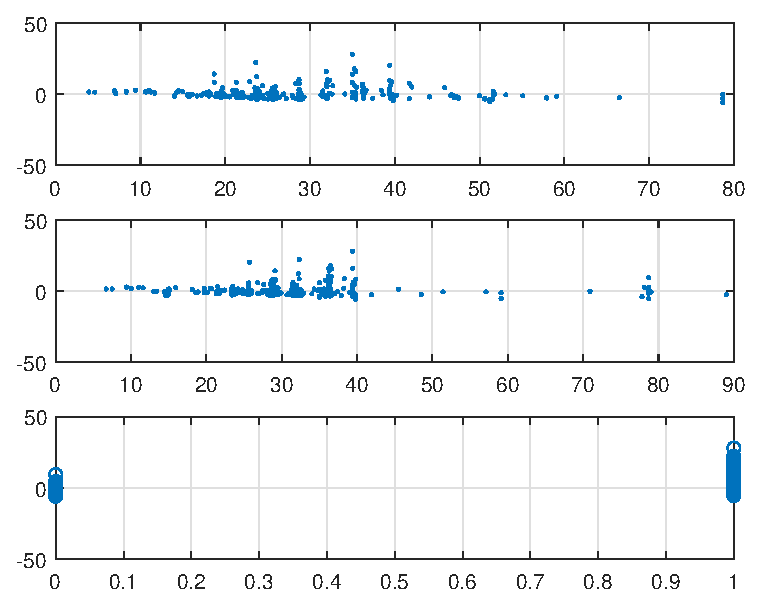
\includegraphics[width=0.55\textwidth]{graphs/fig5.eps}
    \caption{Závislost vysvětlujících proměnných na reziduích}
    \label{fig:lr5}
\end{figure}
\FloatBarrier

\section{Závěr}

V semestrální práci jsme si vyzkoušeli analýzu datasetu a ověření splnění předpokladů pro tvorbu linearního modelu.
Ačkoliv ne všechny výsledky vyšly dle očekávání, lze předpokládat, že hlubší analýzou podstaty dat a dodefinováním příznaků lépe vystihujících jejich pravé vlastnosti by bylo možné docílit lepších výsledků a nápravy vzniklých nesrovnalostí.
